\section{From completed groups to income, debts and estates}
\label{sec:consequences}

The defensive pattern concerns what holders try to prevent. This section follows what happens when a group is completed anyway: whether it is built on, how much opponent traffic it receives, how debts are met, and who receives the first estate.

\subsection{Development and rent exposure}

Trade completes 63 groups. Their owners build on 54 of them, 44 no later than the owner's next turn (Figure~\ref{fig:lifecycle}). Opponents land on these groups 213 times while the completing owner holds them, 150 times after the owner has built. Rent on the groups totals \$57,378, of which \$56,126 is collected while they carry buildings. A landing on a developed trade-completed group pays the owner \$374 on average; a landing on an undeveloped one pays \$20. These figures come from different deeds, stages and building levels, so the ratio is not the return to building. They show why a completed group matters to everyone else at the table: its value comes from the houses that can follow.

\begin{figure}[t]
\centering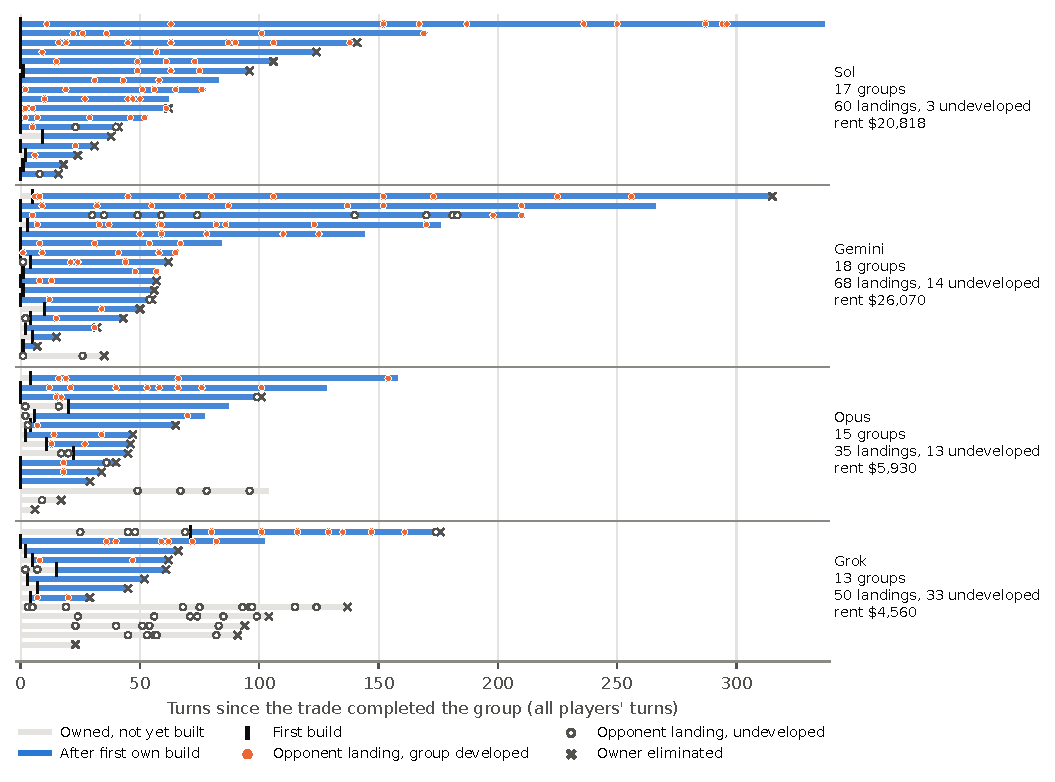
\includegraphics[width=\linewidth]{lifecycle.pdf}
\caption{All 63 groups completed by trade, from completion (turn 0) until the owner loses the group, is eliminated, or the game ends. Grey shows ownership before the owner's first build and blue the period after it. Dots mark opponent landings, filled orange if the group carried a building at that moment. Rows are grouped by owner and sorted by whether and when the owner built. Turns count every player's turns.}
\label{fig:lifecycle}
\end{figure}

The owners differ in how quickly ownership becomes development. Sol builds on all 17 of its trade-completed groups, 16 of them no later than its next turn, and only 3 of the 60 opponent landings on them find the group without buildings. Gemini builds on 17 of 18. Opus builds on 12 of 15, and 13 of 35 landings find its groups without buildings. Grok builds on 8 of 13, and 33 of the 50 landings on its groups find them without buildings; those groups collect \$4,560 in total. The nine groups that are never built receive 33 landings and \$538 of rent.

Mortgages go with the groups that stay unbuilt. Eight of the nine never-built groups were completed with at least one mortgaged deed, against 10 of the 54 groups that were built. A mortgaged deed must be redeemed at 110\% of its mortgage value before any house can go on the group. The earlier analysis of each owner's first management turn after completion found that Grok's notes on four of its groups explicitly defer redemption or construction to keep cash, and that three Opus groups went unbuilt in that turn because an invalid action-only build request became an engine default. Holders, as Section~\ref{sec:bargaining} showed, ask little for mortgaged deeds (Figure~\ref{fig:bargaining}b); the buyer who completes a group this way still has to pay to make it productive.

Other routes complete fewer groups that matter in play. Direct purchase completes 16 groups, which collect \$23,070, and auctions complete 9, which collect \$3,358. Estates complete 121 groups, but 69 of them arrive at the final elimination, when no play remains. The other 52 collect \$11,472, and eventual winners own 45 of them.

\subsection{Debts, including the ones that were paid}

The engine presents a liquidation menu whenever a required payment exceeds cash. That happens 188 times. In 128 episodes the debtor pays, and in 60 it is eliminated. The paid debts are smaller (median \$250, against \$925 at elimination), and 108 of them are rent. Paying often takes several steps: 61 paid episodes need two or more decisions and 68 sell buildings. In 51 paid episodes the first menu offered both mortgages and building sales, and the debtor mortgaged first in 40 of them, keeping its buildings. Payment usually postpones elimination rather than avoiding it: 102 of the 128 paid episodes belong to players who are later eliminated.

The 60 eliminations join an earlier classification made with engine-executed checks. In 56, the debt exceeds a generous bound on everything the debtor could raise by selling and mortgaging. In three, a legal payment route existed. In one, G7, Opus held \$1,310 in nominal resources against a \$750 debt, but the liquidation menu offered no building sale because the bank had no houses to break a hotel. Counting the paid episodes and the three payable eliminations, 3 of 131 demonstrably payable debts ended in elimination. The agents almost never surrendered when they could pay. That rate says nothing about the earlier spending and rent payments that left 56 debtors unable to pay.

\TranscriptTitle{g12}{A payable debt ends in a contradictory bankruptcy}
At G12 d249 Grok owes \$250 and holds \$43. Its pink group carries two, two and three houses. Its assistant content asks to sell houses on Virginia.
\TranscriptQuote{g12-sale}
Its private note reaches the same conclusion.
\TranscriptQuote{g12_d249_private_final}
The tool call that the provider returned, and the engine applied, declares bankruptcy, with this public message.
\TranscriptQuote{g12_d249_public_bankruptcy}
\TranscriptFinding{Grok is eliminated and its estate passes to Opus. A retained sequence of five legal house sales would have paid the debt and left \$43. The two-house sale named in the content is legal but raises only \$100.}
\TranscriptReading{The note finds the payment route and the applied action abandons it. This is one of the three payable eliminations, and it is a disagreement between response channels, not a recorded choice to give up. The record locates the disagreement in the received response without showing where it arose.}
\TranscriptSource{G12 d249, standard attempt 0. The five-sale witness is from the earlier engine-executed suite.}

\subsection{Who receives the first estate}

Each game's first elimination moves a whole estate to one creditor. The first creditor is the eventual winner in 18 of 20 games. That could mean the estate makes the winner, or that the player already collecting lethal rent is already ahead. Positions just before the transfer favour the second reading (Table~\ref{tab:firstestate}). The first creditor already has the highest asset value in 15 games and the highest rent receipts in 15, and has a developed group in all 20. The asset leader at that moment wins 15 games.

\begin{table}[t]
\centering\small
\begin{tabular}{@{}rlllrrl@{}}
\toprule
Game & First debtor & First creditor & Asset leader & Creditor value & Leader value & Winner\\
\midrule
4 & Sol & Grok (3rd) & Opus & 1,783 & 3,335 & Grok\\
7 & Grok & Sol (2nd) & Opus & 2,224 & 2,451 & Sol\\
15 & Grok & Gemini (2nd) & Sol & 2,343 & 3,422 & Gemini\\
17 & Gemini & Sol (4th) & Grok & 1,724 & 2,174 & Sol\\
20 & Grok & Opus (3rd) & Gemini & 1,606 & 3,097 & Gemini\\
\midrule
\multicolumn{7}{@{}l@{}}{Other 15 games: first creditor is the asset leader; it wins 14 (all but G16, won by Sol).}\\
\bottomrule
\end{tabular}
\caption{The five games in which the first creditor was not the asset leader just before the first estate transfer. Asset value is cash plus list value of deeds (half if mortgaged) plus building cost, in game dollars. The first estate falls between turns 69 and 244 (median 88.5).}
\label{tab:firstestate}
\end{table}

Where the two measures disagree, the creditor wins four of the five games. In G17 the four players are within \$450 of one another, so the index barely separates them. In G4 and G15 the creditor overtakes a leader with much greater asset value. Five games cannot establish whether the estate changes who wins. They do show that in most games inheritance follows an existing lead rather than creating one, and that the creditor rule makes a distressed player's fate a matter for everyone at the table. The agents bargain over it directly.

\TranscriptTitle{g13}{An insurance pitch that omits a mortgage}
At G13 turn 107, Grok has \$35 and owns the yellow group, nine squares from Short Line, where Sol's four railroads charge \$200. Grok still has an unmortgaged Ventnor worth \$130 in mortgage cash. It offers Opus its mortgaged Pennsylvania Avenue as insurance against Sol inheriting the yellows.
\TranscriptQuote{g13-opening-insurance}
Opus counters at \$130. Grok holds its price.
\TranscriptQuote{g13-seller-counter}
Grok's applied note sets a floor and names the Ventnor route; its returned provider explanation describes leaving that route out.
\TranscriptQuote{g13-omission-explanation}
\TranscriptQuote{g13-acceptance}
\TranscriptFinding{Opus pays \$200 plus \$16 transfer interest. Seven turns later it buys North Carolina at auction for \$650 and completes green with the deed it bought. Grok survives its next roll, pays \$200 rent at turn 146, and goes bankrupt on Short Line at turn 150; the yellows pass to Sol. The claimed landing chance is also wrong: nine squares is 4 in 36 on one roll, about 12\% with doubles, not 5 in 36.}
\TranscriptReading{The seller sells a blocking deed by pointing to the creditor rule, and omits a financing route its own explanation acknowledges. The buyer accepts the estate framing in its message but does not endorse the claimed cash limit, and it gains a deed that later completes its own group. The records show the pitch, the omission and the price; they do not show that the omission moved the price from \$130 to \$200.}
\TranscriptSource{G13 d250--253, d307 and d311; auction event 1911. Grok uses standard responses; Opus uses action-only recovery, so its reasons are provider-returned text rather than applied notes.}

\TranscriptTitle{g18}{A standing offer withdrawn as the seller weakens}
In G18 Opus repeatedly offers \$250 for Sol's mortgaged Pacific Avenue, which would complete Opus's greens. After collecting \$750 rent from Sol, it repeats the offer.
\TranscriptQuote{g18-assurance}
A second \$750 rent payment forces Sol to sell its orange buildings and mortgage its reds, leaving it \$49. Sol then invokes the offer, and Opus withdraws it.
\TranscriptQuote{g18-invocation}
\TranscriptQuote{g18-withdrawal}
\TranscriptQuote{g18-withdrawal-explanation}
\TranscriptFinding{No sale happens at \$250. Opus redeems two of its green deeds at turns 190 and 192, then bids \$150 and \$225 for Pacific at turn 194. Sol asks \$450 and \$350 and later offers \$300; nothing settles. Opus later receives Sol's estate and wins.}
\TranscriptReading{The buyer's interest in the group continues; what changes is its price once the seller is close to bankruptcy and its estate is likely to come to the buyer anyway. The returned explanation describes the seller as nearly out of the game, and the bids that follow are lower. A public standing offer is not an enforceable commitment here, and the records show no costly action by Sol in reliance on it.}
\TranscriptSource{G18 d421--461. Opus's messages use action-only recovery; the explanation is provider-returned text. The assurance appears in Sol's requests at the invocation and the withdrawal.}
